\documentclass[11pt]{article}
\usepackage{fontspec}
\usepackage[a4paper,margin=2.3cm]{geometry}
\usepackage{graphicx}
\usepackage{booktabs}
\usepackage{array}
\usepackage{xcolor}
\usepackage{float}
\usepackage{fancyvrb}
\usepackage[hidelinks]{hyperref}

\setmainfont{Helvetica Neue}
\setmonofont{Menlo}
\renewcommand{\arraystretch}{1.25}

\title{\textbf{Athena TTS — Báo cáo so sánh 5 engine TTS}\\[2pt]
\large Dữ liệu thô \& biểu đồ (không kết luận)}
\author{}
\date{15/06/2026}

\begin{document}
\maketitle
\vspace{-1.5em}

\section*{1. Tổng quan}
Năm engine TTS mã nguồn mở (Kokoro, Chatterbox, F5-TTS, StyleTTS2, IndexTTS2) chạy trên
cùng cấu hình (CPU, Apple M4 Pro). Hai bài test:
\begin{itemize}\setlength\itemsep{1pt}
\item \textbf{Test A — chỉ số âm học} trên kịch bản 1 (9 câu).
\item \textbf{Test B — độ giống giọng gốc} trên kịch bản 2 (6 câu), cùng file mẫu \texttt{refs/speaker.wav} (11s).
\end{itemize}
Bốn engine nhân bản giọng từ \texttt{refs/speaker.wav}; Kokoro dùng giọng cài sẵn (không clone).
\textbf{Giọng gốc} (người thật, đọc kịch bản 1, 40.3s, trích từ \texttt{original\_voice.wav})
được đưa vào làm mốc tham chiếu. Tài liệu này chỉ trình bày số đo và biểu đồ.

\section*{2. Hai kịch bản được test}
\textbf{Kịch bản 1 (Test A):}
\begin{Verbatim}[frame=single,fontsize=\footnotesize,rulecolor=\color{gray}]
Hello, this is a short voice consistency test.
Please keep the same tone, speed, and energy throughout the recording.
The quick brown fox jumps over the lazy dog.
Today is June fifteenth, twenty twenty-six.
I will now repeat one sentence three times.
The product sounds clear, stable, and natural.
The product sounds clear, stable, and natural.
The product sounds clear, stable, and natural.
End of test. Thank you.
\end{Verbatim}
\textbf{Kịch bản 2 (Test B):}
\begin{Verbatim}[frame=single,fontsize=\footnotesize,rulecolor=\color{gray}]
The morning train arrived exactly on time today.
She carefully placed the old letters back into the wooden box.
Could you please tell me how to get to the central library?
Numbers like seven, nineteen, and forty-two appear quite often.
Honestly, I did not expect the final results to be this good.
Thank you for listening, and I hope you have a wonderful day.
\end{Verbatim}

\section*{3. Cơ chế từng engine}
\begin{table}[H]\centering\small
\begin{tabular}{>{\bfseries}l l p{9.2cm}}
\toprule
Engine & Kiểu & Cơ chế \\
\midrule
Kokoro & Non-autoreg. (82M) & Mô hình nhỏ, sinh thẳng một lần. Giọng cài sẵn (style vector). Không nhân bản giọng. \\
Chatterbox & Tự hồi quy (LM) & Transformer kiểu Llama (0.5B) sinh ``token âm thanh'' lần lượt từ văn bản + giọng mẫu, rồi vocoder dựng sóng. Có tham số cảm xúc. \\
F5-TTS & Flow-matching (DiT) & Diffusion Transformer, sinh song song. ``Điền'' giọng dựa trên audio mẫu + văn bản qua nhiều bước; vocoder Vocos. \\
StyleTTS2 & Style diffusion + GAN & Diffusion sinh ``style vector'', kèm bộ dự đoán thời lượng/ngữ điệu và decoder kiểu HiFi-GAN; huấn luyện đối kháng. Clone zero-shot. \\
IndexTTS2 & Tự hồi quy (GPT) & GPT sinh token ngữ nghĩa; semantic codec (w2v-BERT + MaskGCT), embedding người nói (CAMPPlus), cảm xúc (Qwen), rồi flow $\rightarrow$ mel + vocoder BigVGAN. \\
\bottomrule
\end{tabular}
\end{table}

\section*{4. Thời gian tạo (CPU, model đã cache)}
Đo tuần tự (không chạy song song); gồm thời gian nạp model + suy luận.
\begin{table}[H]\centering
\begin{tabular}{l r r}
\toprule
Engine & Thời gian (giây) & Độ dài audio (giây) \\
\midrule
Kokoro & 12.7 & 29.4 \\
StyleTTS2 & 29.5 & 39.4 \\
Chatterbox & 38.0 & 33.4 \\
IndexTTS2 & 68.8 & 25.2 \\
F5-TTS & 253.7 & 37.4 \\
\bottomrule
\end{tabular}
\end{table}

\section*{5. Test A — Chỉ số âm học (kịch bản 1)}
Các đại lượng đo (mỗi cột là một số đo khách quan, không diễn giải):
\begin{itemize}\setlength\itemsep{0pt}
\item \texttt{f0\_mean} cao độ trung bình (Hz); \texttt{f0\_std} độ lệch chuẩn cao độ (Hz).
\item \texttt{f0\_range} khoảng cao độ p5--p95 (Hz); \texttt{f0\_st\_std} dao động cao độ theo semitone.
\item \texttt{energy\_dB} biến thiên năng lượng trong phần có tiếng (dB).
\item \texttt{pause/s} số lần ngắt nghỉ ($>$150\,ms) mỗi giây; \texttt{voiced} tỉ lệ khung có thanh.
\item \texttt{centroid} trọng tâm phổ (Hz) — liên quan độ sáng của tone.
\end{itemize}
\begin{table}[H]\centering\small
\begin{tabular}{l r r r r r r r r}
\toprule
Engine & f0\_mean & f0\_std & f0\_range & f0\_st\_std & energy\_dB & pause/s & voiced & centroid \\
\midrule
\textbf{Giọng gốc} & \textbf{182.7} & \textbf{90.8} & \textbf{275.7} & \textbf{10.4} & \textbf{10.2} & \textbf{0.35} & \textbf{0.68} & \textbf{2722.9} \\
\midrule
Kokoro & 211.3 & 36.1 & 121.6 & 2.82 & 10.9 & 0.34 & 0.51 & 3374.7 \\
Chatterbox & 250.4 & 71.1 & 213.1 & 4.82 & 9.83 & 0.36 & 0.65 & 2924.0 \\
F5-TTS & 165.3 & 82.2 & 249.6 & 9.35 & 17.7 & 0.35 & 0.69 & 3093.3 \\
StyleTTS2 & 204.4 & 36.3 & 111.6 & 2.93 & 9.87 & 0.36 & 0.54 & 2749.4 \\
IndexTTS2 & 232.0 & 62.2 & 188.2 & 4.42 & 8.72 & 0.44 & 0.47 & 2592.3 \\
\bottomrule
\end{tabular}
\end{table}

\noindent Điểm proxy 0--1 cho từng tiêu chí (chuẩn hoá quanh giá trị tự nhiên của giọng người;
\texttt{TOTAL} là tổng có trọng số, thang 0--100). Đây là chỉ số tính toán, để tham khảo:
\begin{table}[H]\centering\small
\begin{tabular}{l r r r r r r r}
\toprule
Engine & intonation & pitch\_range & energy & phrasing & voicing & timbre & TOTAL \\
\midrule
\textbf{Giọng gốc} & 0.00 & 0.04 & 0.97 & 0.97 & 0.87 & 0.95 & 51.7 \\
\midrule
StyleTTS2 & 0.80 & 0.86 & 0.98 & 0.98 & 0.92 & 0.94 & 89.6 \\
IndexTTS2 & 0.91 & 0.74 & 1.00 & 0.99 & 0.68 & 0.99 & 89.5 \\
Kokoro & 0.76 & 0.92 & 0.92 & 0.96 & 0.85 & 0.48 & 80.9 \\
Chatterbox & 0.69 & 0.44 & 0.99 & 0.98 & 0.94 & 0.84 & 78.4 \\
F5-TTS & 0.00 & 0.13 & 0.19 & 0.97 & 0.83 & 0.71 & 35.4 \\
\bottomrule
\end{tabular}
\end{table}

\noindent\textit{Ghi chú về chỉ số:} điểm proxy \texttt{intonation}/\texttt{pitch\_range} được
chuẩn hoá quanh mức $\sim$4 semitone (giọng đọc thông thường); giọng gốc dao động tới 10.4 st nên
bị hai điểm này thấp. Hãy đối chiếu trực tiếp \textbf{số đo thô} và biểu đồ dưới đây thay vì chỉ nhìn \texttt{TOTAL}.

\begin{figure}[H]\centering
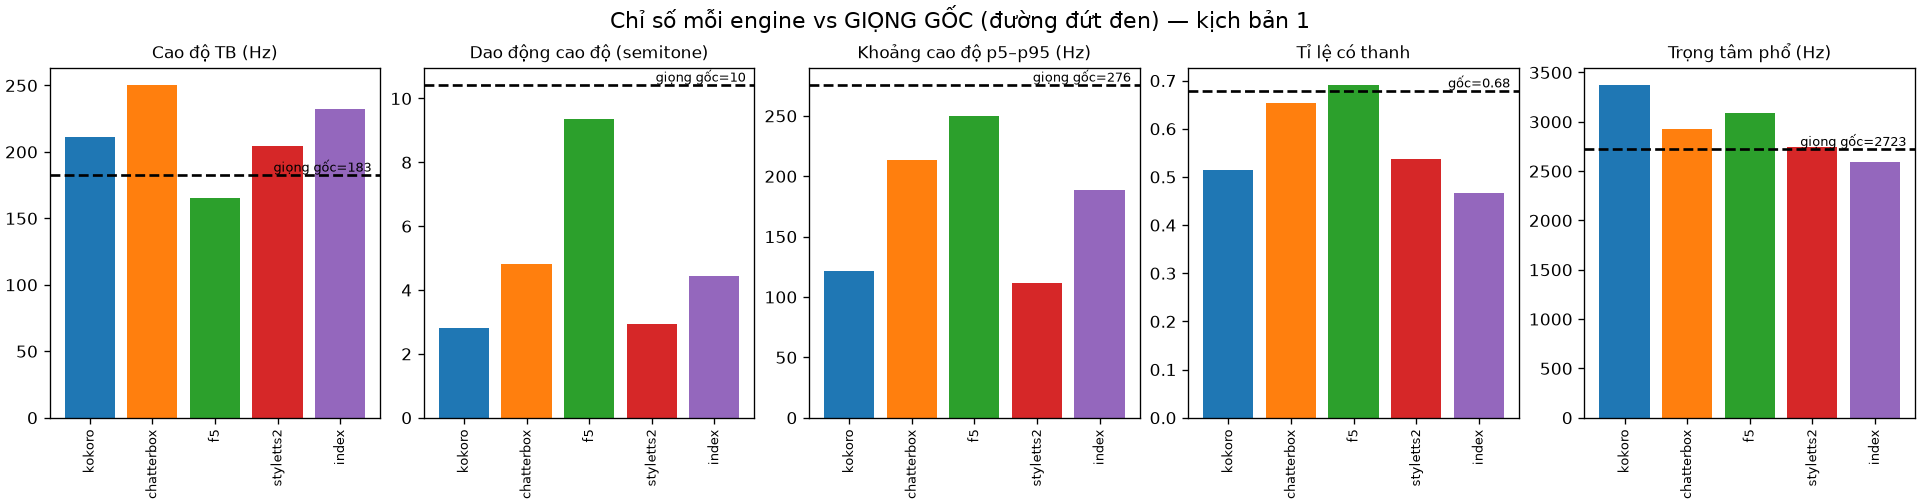
\includegraphics[width=\linewidth]{compare_to_original.png}
\caption{Từng chỉ số của mỗi engine (cột màu) so với GIỌNG GỐC (đường đứt đen).
Trục hoành: 5 engine. Trục tung: giá trị chỉ số (đơn vị ghi trên tiêu đề mỗi ô).
Cột càng gần đường đứt = càng giống giọng gốc ở chỉ số đó.}
\end{figure}

\begin{figure}[H]\centering
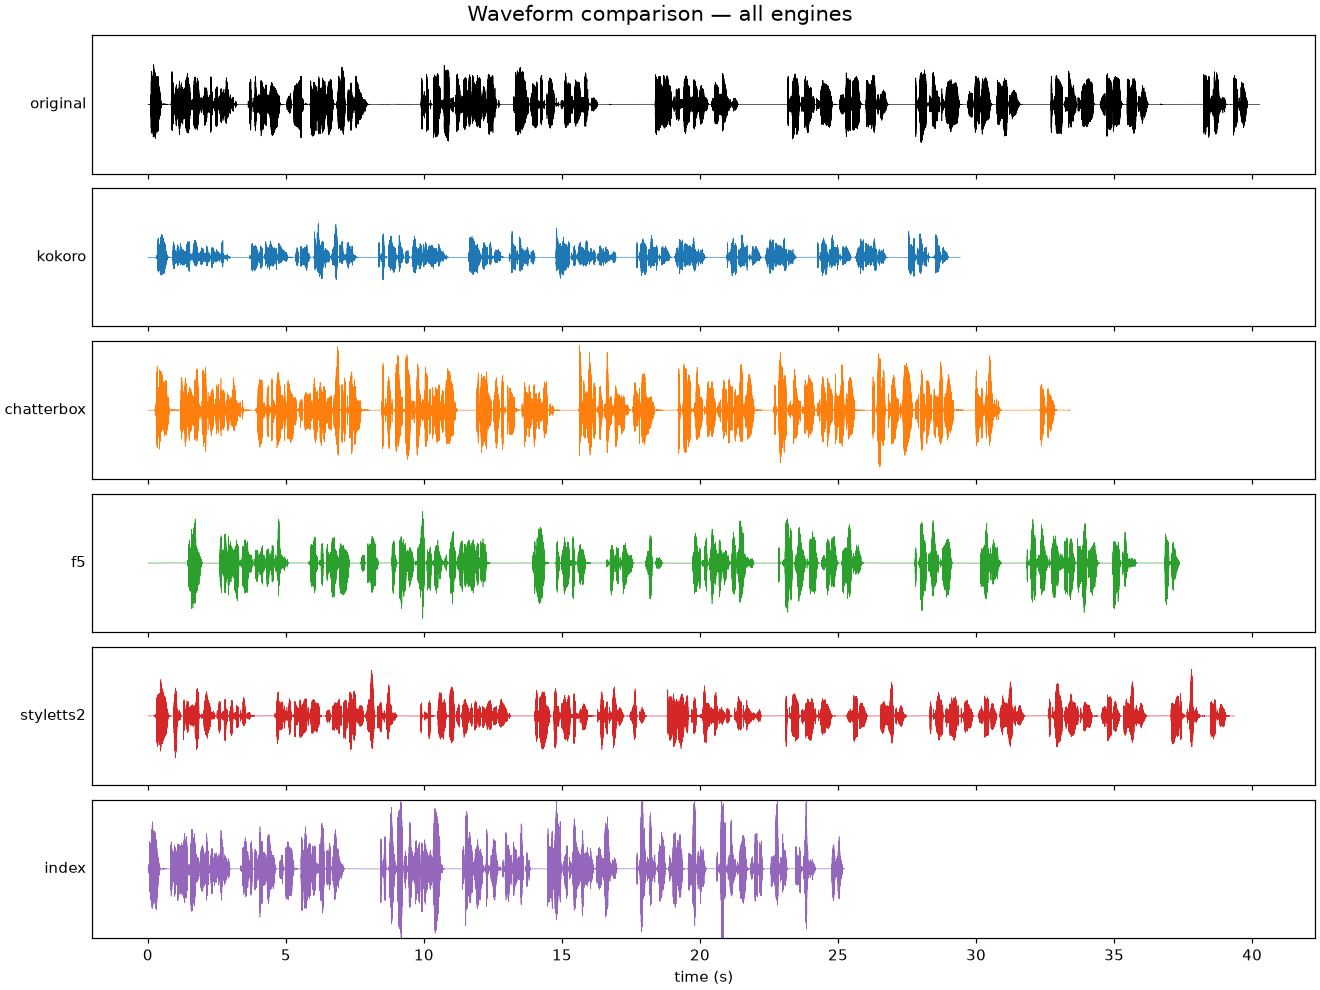
\includegraphics[width=\linewidth]{compare_waveforms.png}
\caption{Biểu đồ sóng (kịch bản 1). Trục hoành: thời gian (giây).
Trục tung: biên độ tín hiệu (chuẩn hoá $[-1,1]$). Mỗi hàng là một engine.}
\end{figure}

\begin{figure}[H]\centering
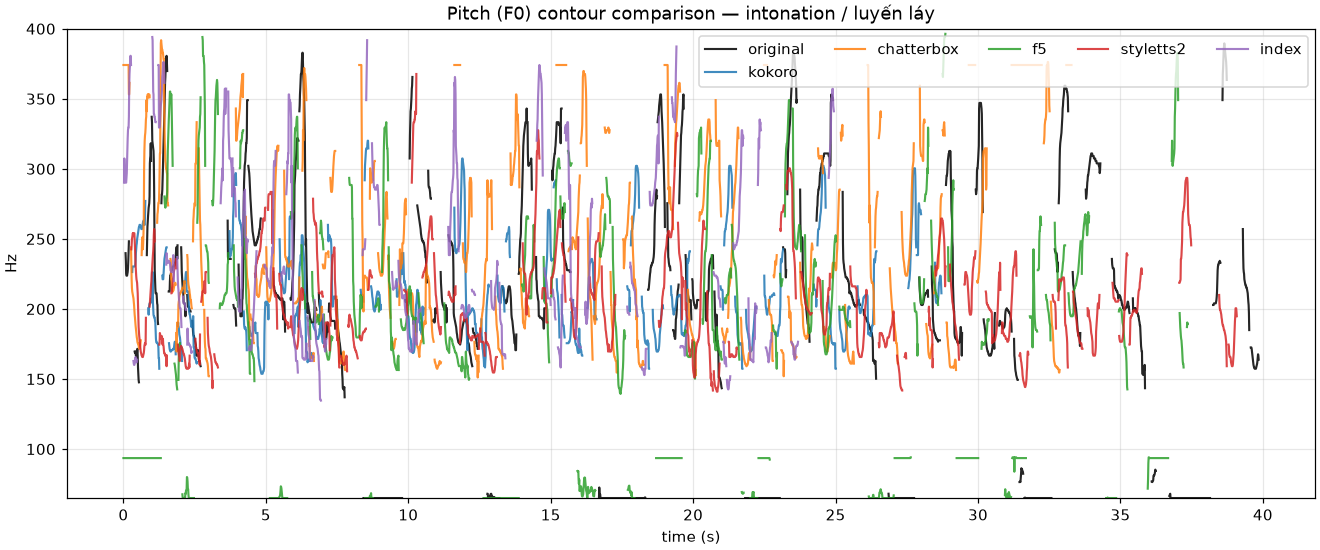
\includegraphics[width=\linewidth]{compare_pitch.png}
\caption{Đường cao độ F0 (kịch bản 1). Trục hoành: thời gian (giây).
Trục tung: cao độ cơ bản F0 (Hz). Mỗi màu là một engine; \textbf{màu đen = giọng gốc}.}
\end{figure}

\section*{6. Test B — Độ giống giọng gốc (kịch bản 2)}
Cách đo: trích \textit{speaker embedding} bằng Resemblyzer (d-vector GE2E), tính
\textbf{cosine similarity} giữa output mỗi engine và giọng gốc \texttt{refs/speaker.wav}
(thang 0--1). \textbf{Trần = 0.983}: cosine giữa hai clip khác nhau của cùng một người
(\texttt{speaker.wav} và \texttt{speaker\_full.wav} — đều trích từ \textbf{giọng gốc}).
\begin{table}[H]\centering
\begin{tabular}{>{\bfseries}l r r l}
\toprule
Engine & Cosine & \% so với trần & Nhân bản giọng \\
\midrule
F5-TTS & 0.969 & 99\% & Có \\
IndexTTS2 & 0.966 & 98\% & Có \\
Chatterbox & 0.953 & 97\% & Có \\
StyleTTS2 & 0.923 & 94\% & Có \\
Kokoro & 0.832 & -- & Không (giọng cài sẵn) \\
\bottomrule
\end{tabular}
\end{table}

\begin{figure}[H]\centering
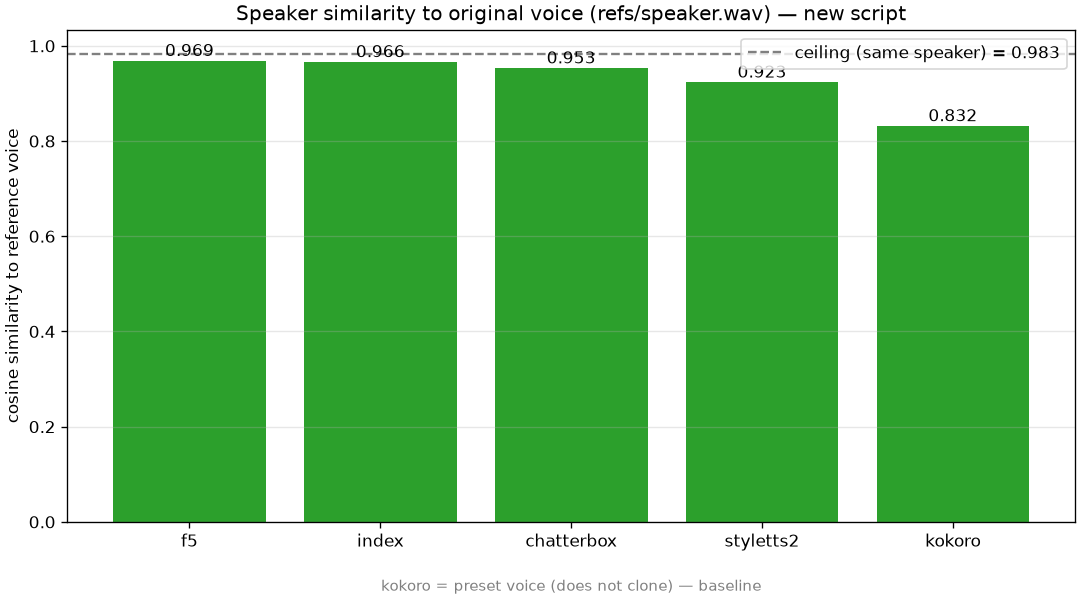
\includegraphics[width=0.9\linewidth]{similarity_chart.png}
\caption{Trục tung: cosine similarity với giọng gốc (0--1, càng cao càng giống).
Mỗi cột là một engine. Đường gạch ngang: mức trần 0.983 (cùng người).}
\end{figure}

\begin{figure}[H]\centering
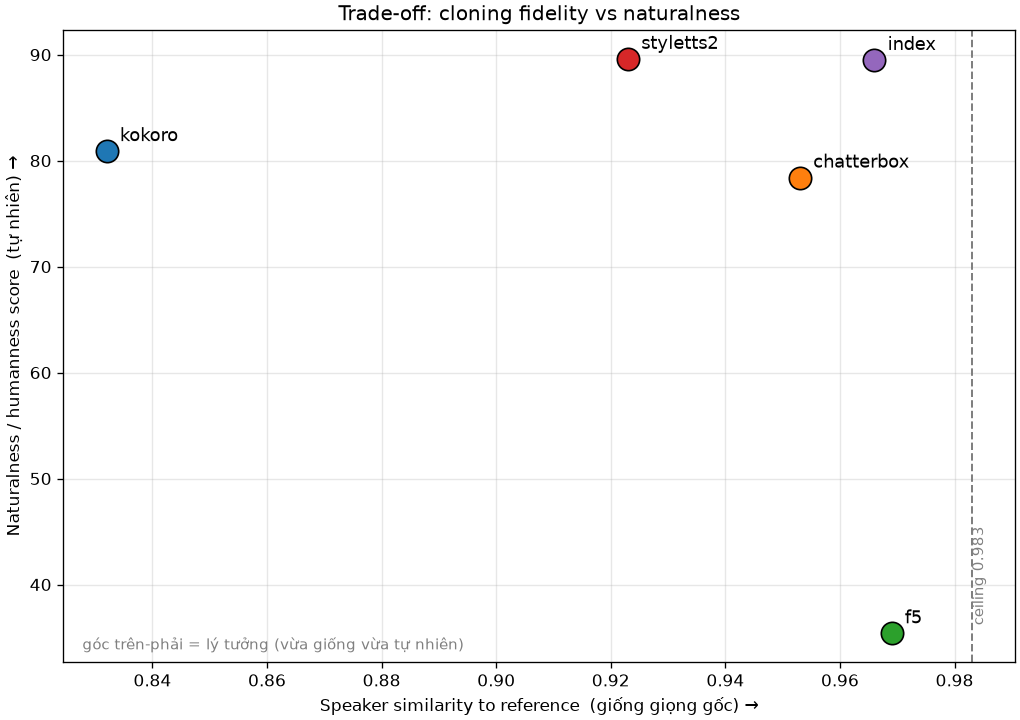
\includegraphics[width=0.8\linewidth]{tradeoff_scatter.png}
\caption{Trục hoành: độ giống giọng gốc (cosine similarity, Test B).
Trục tung: điểm độ tự nhiên \texttt{TOTAL} (0--100, Test A).
Mỗi điểm là một engine. Đường gạch dọc: mức trần cosine 0.983.}
\end{figure}

\begin{figure}[H]\centering
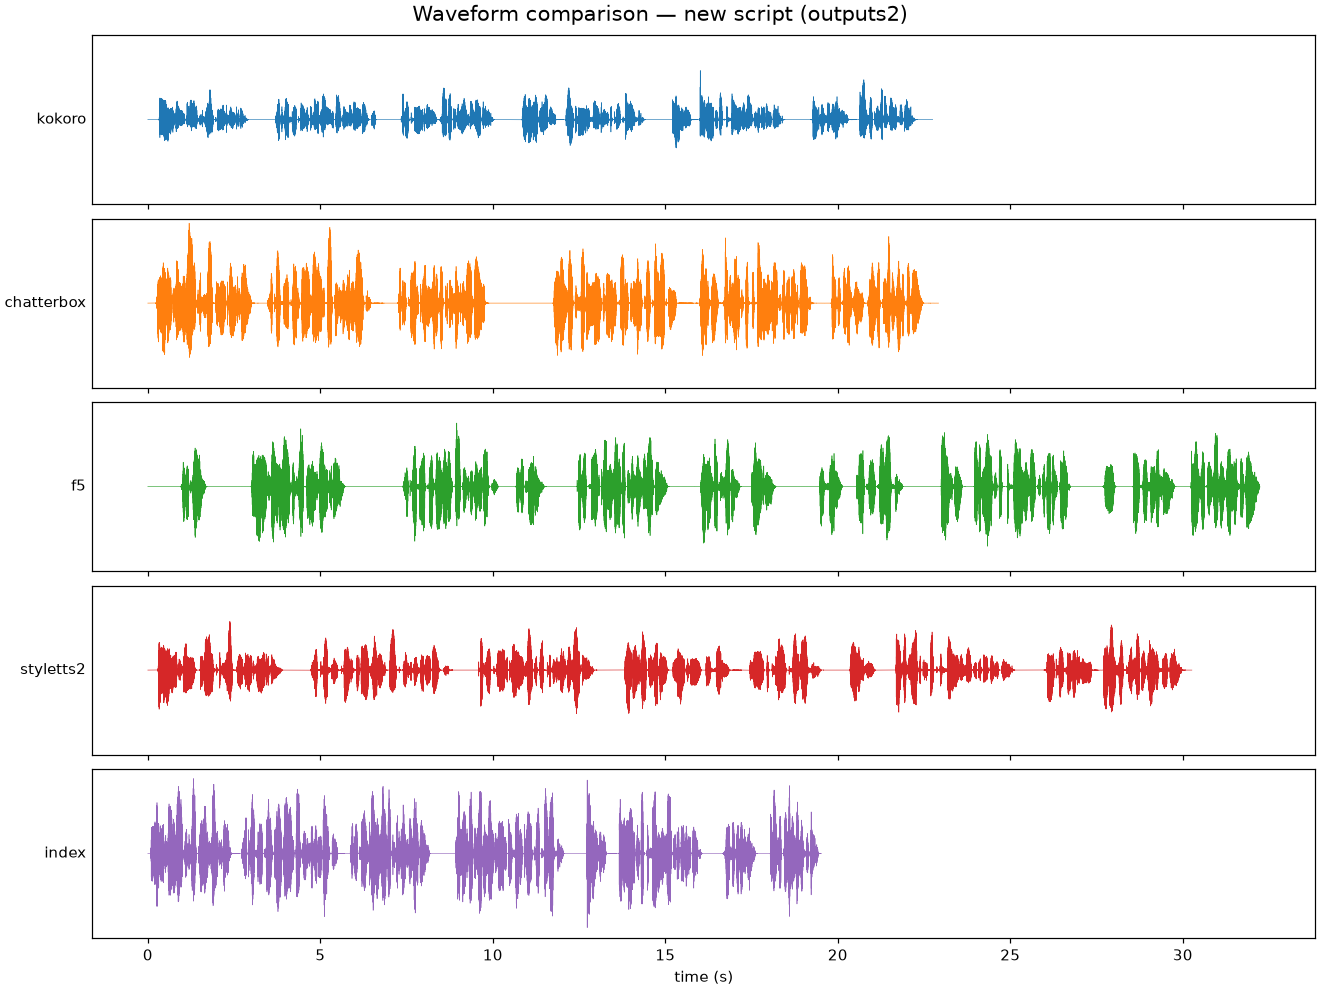
\includegraphics[width=\linewidth]{compare_waveforms2.png}
\caption{Biểu đồ sóng (kịch bản 2). Trục hoành: thời gian (giây).
Trục tung: biên độ tín hiệu (chuẩn hoá $[-1,1]$). Mỗi hàng là một engine.}
\end{figure}

\begin{figure}[H]\centering
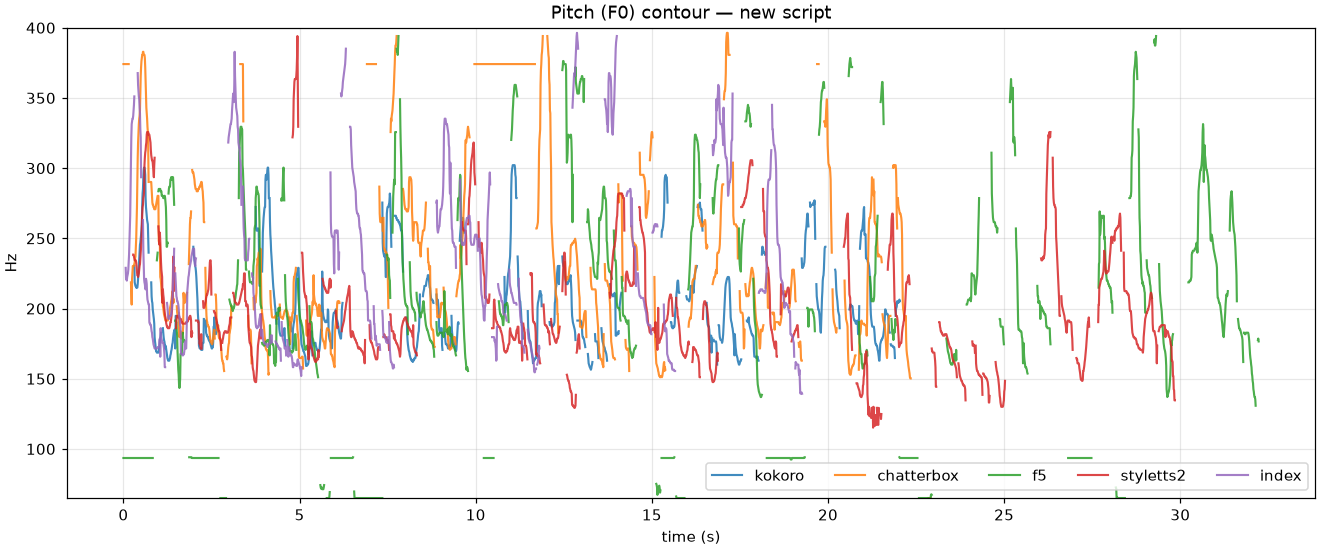
\includegraphics[width=\linewidth]{compare_pitch2.png}
\caption{Đường cao độ F0 (kịch bản 2). Trục hoành: thời gian (giây).
Trục tung: cao độ cơ bản F0 (Hz). Mỗi màu là một engine.}
\end{figure}

\end{document}
